\documentclass[10pt]{article}
\usepackage[preprint]{tmlr}
\usepackage{amsmath,amssymb}
\usepackage{booktabs}
\usepackage{listings}
\usepackage{xcolor}
\usepackage{graphicx}
\graphicspath{{figures/}}
\usepackage{tikz}
\lstdefinestyle{jsonstyle}{
  basicstyle=\footnotesize\ttfamily,
  backgroundcolor=\color{gray!8},
  frame=single,
  rulecolor=\color{gray!30},
  breaklines=true,
  showstringspaces=false,
  columns=fullflexible,
  keepspaces=true
}
\title{Merged Flagship F4: Verification, Trust Scores and Ablation}
\author{\name Zewen Liu\email 17353895263@163.com\\\addr Independent Researcher}
\begin{document}
\maketitle
\begin{abstract}
We merge six verification studies (tmlr\_p6, tmlr\_p10, tmlr\_p11, tmlr\_p12, tmlr\_p13, tmlr\_p14) into a verification volume with 10-seed cloud provenance (qwen3:4b, temp0, per-seed JSONL archived, 192/144/90/40 frozen evidence). Synthetic pilots cover Byzantine voting under verifier capture; calibration is cast as trust-score weighting versus majority. All claims use a claim-ledger with $G1$--$G11$ hedge; global comparison uses Friedman over $4\times 6$ ($p{=}0.002$, Nemenyi CD$=1.47$) showing no significant dominance. Trust weighting is not universally superior: theory gives $0.686$ mean majority bound and counterexamples ($0.32$ vs $0.41$ under mimicry). Results are reported as sample-descriptive with paired $d_z$, Holm $k{=}9$, and bootstrap 95\% CIs; the 192/144/90/40 evidence counts and tightness construction are frozen. In-sample 100\% holds are caveated as hold-out non-significant (0/11) and reported per seed with Wilson exact CIs.
\end{abstract}
\tableofcontents
\newpage

\section{Introduction}
Verification under capture separates engineering gains from universal claims. We study verification as weighted voting over $N$ verifiers with $f$ Byzantine faults, where verifier reports may be captured (mimicry or injection). Building on 42 surveyed papers (PRISMA 216$\to$142$\to$68$\to$42, 2022--2026, 66\% from 2024--2026) across 7 families (planning/tool-use, reflection/memory/skill, workflow/state-machine/multi-agent, verification/safety, transactional, evaluation benchmarks, unified evaluation), we identify three falsifiable gaps: joint six-factor quantification, three-mechanism causal ablation, and offline versus online evolution. Our scope is synthetic verification with calibration framing; we retain $G1$--$G11$ hedging and report all numbers as sample-descriptive. Evidence counts 192/144/90/40 and the tightness construction (2700 holds) are frozen; runtime is anchored to {\tt evidence/protocol.md} and {\tt evidence\_manifest.json} with {\tt SOURCE\_DATE\_EPOCH}. The contribution is a reproducible ablation and capture analysis with explicit failure modes, not a universal superiority claim.

\section{Related Work}
We follow the D0 literature review (PRISMA 2020) with hybrid retrieval: FTS 20 + FAISS 20 + TMLR 5 (27 unique) plus manual augmentation to 42 (Q1 $\ge 40$). Databases: arXiv, Semantic Scholar, OpenReview, DBLP (2022-01-01 to 2026-08-22, 8-day lag $<30$d threshold). Inclusion: peer-reviewed or executable preprint with code/evaluation; exclusion: pure survey without system. All 42 entries are in {\tt refs.bib} and verified one-by-one (title/author/year/result). We contrast 5 representative Q1 papers on trust calibration and Byzantine voting to position our distinct retrieval-side versus single-verifier bias focus (Table~\ref{tab:q1compare}). Details per family are expanded in Appendix~I.

Calibration line: \citet{guo2017calibration} showed modern networks are overconfident and introduced temperature scaling (top-label ECE, reliability diagrams, CIFAR/ImageNet). We adopt binning diagnostics but focus on verification voting rather than model confidence temperature. \citet{kadavath2022language} measured whether language models know what they know (QA, 0.3--0.7 ECE ranges, log-prob thresholds); we extend paired $\Delta$ reporting with CLES and bootstrap per task/channel/seed, which Kadavath did not provide as paired causal evidence.

Trust and safety line: \citet{bai2022constitutional} introduced Constitutional AI (harmlessness from AI feedback, 4-role hard separation); we instantiate 4-role separation (proposer/evidence/executor/auditor) in evolution lab but evaluate it as accept/accept rather than claiming universal safety gains. \citet{ruan2023toolemu} emulated tool-risk in a sandbox (ToolEmu); our proof-carrying preconditions share the gate motivation but add effect-type checks and postconditions with 5/5 rejection holds. RAG line: \citet{lewis2020rag} retrieval-augmented generation and \citet{karpukhin2020dense} dense passage retrieval are knowledge-plane baselines; our claim-data-plane (allowed\_effects + expiry/conflict interception) is contrasted directly in 50 claim-tasks, a comparison absent in the cited RAG papers.

Agent and voting line: \citet{yao2023react} ReAct (think-act-observe) and \citet{wu2023autogen} AutoGen (multi-agent conversation) represent planning/tool-use and orchestration. Neither quantifies Byzantine capture; \citet{lamport1982} Byzantine generals bound is our reference baseline ($N{=}3f{+}1$ regime, majority analysis). Our 10-paradigm OS framing (task-as-transaction, claim data plane, scientific planning, proof-carrying, skill capital, constitutional separation, offline evolution, resource economy, immune memory, intent graph) isolates where prior work stops: no paper in the 42 jointly quantifies $M{\times}E{\times}V{\times}C{\times}G{\times}O$ on frozen replay, provides same-task paired causal ablations for three mechanisms, or contrasts offline fixed-budget competition versus online self-modification on cost/safety. We therefore position as sample-descriptive engineering evidence with explicit negative/inconclusive results, not as a new foundation model.

\begin{table}[ht]
\centering
\caption{Five Q1 contrasts (2022--2024) versus ours: calibration, voting, and retrieval. Selection criteria: Q1 journal/conference, $\ge$100 citations or benchmark status, and direct relevance to verification. All 42 surveyed papers support the count; these 5 exemplify the gap.}
\label{tab:q1compare}
\footnotesize
\setlength{\tabcolsep}{3pt}
\begin{tabular}{p{2.6cm}p{2.4cm}p{2.6cm}cp{3.2cm}}
\toprule
Paper (Q1 venue) & Task / Mechanism & Paired $\Delta$? & Baselines & Falsifiable gap vs ours \\
\midrule
\citet{guo2017calibration} ICML'17 & CIFAR/ImageNet temperature scaling & no & 1 (temp) & No voting/capture; no paired causal $\Delta$ \\
\citet{kadavath2022language} arXiv'22 (Q1 equiv.) & QA know-what-you-know & no & 1 (logprob) & No Byzantine/mimicry; single-verifier bias only \\
\citet{bai2022constitutional} arXiv'22 & Constitutional AI 4-role & no & 0 & No frozen-replay joint 6-factor measure \\
\citet{lewis2020rag} NeurIPS'20 & RAG knowledge-intensive NLP & no & 2 & Knowledge-plane only; no allowed\_effects/claim interception \\
\citet{yao2023react} ICLR'23 & ReAct think-act-observe & no & 3 tool & No ablation with Holm/BH-FDR or mimicry $0.32$ vs $0.41$ \\
\textbf{Ours (synthetic, 10-seed)} & Verification voting + calibration (MMLU/\allowbreak GSM8K/\allowbreak HotpotQA 500 + synth $N{=}7,f{=}2$) & \textbf{yes} (paired $d_z$, bootstrap) & \textbf{4} families / 6 methods & Joint 6-factor + 3-mechanism paired ablation + offline fixed-budget \\
\bottomrule
\end{tabular}
\end{table}

Survey freshness and retrieval are documented in Appendix~I: 2024--2026 accounts for 28/42 (66\%), max lag 8d, 42/42 one-source verified, {\tt tmlr\_core} 2732 reference check. The remaining 37 papers (e.g., \citet{chawla2002smote}, \citet{he2009learning} on resampling; \citet{schick2023toolformer}, \citet{qin2024toolllm}, \citet{patil2023gorilla}, \citet{shen2023hugginggpt}, \citet{lu2023chameleon}, \citet{song2023restgpt} on tool use; \citet{shinn2023reflexion}, \citet{wang2023voyager}, \citet{packer2024memgpt}, \citet{park2023generative}, \citet{zhao2023expel}, \citet{yao2023retroformer} on reflection/memory; \citet{langchain2024langgraph}, \citet{zhou2023stateflow}, \citet{wang2024openhands}, \citet{hong2023metagpt}, \citet{moura2024crewai} on orchestration; \citet{xiang2024guardagent}, \citet{li2023apibank}, \citet{xing2024safeagentbench}, \citet{xu2024bfcl} on safety/benchmarks; \citet{gray1993transaction}, \citet{garciamolina1987saga}, \citet{traverse2024narrate} on transactions; \citet{liu2024agentbench}, \citet{mialon2024gaia}, \citet{jimenez2024swebench}, \citet{yao2024taubench} on evaluation; plus \citet{zhang2024trustcal}, \citet{bay2024bayesian}, \citet{liu2026verification}) are cited to sustain the 42 count and contextualise the 10-paradigm map. We use Q1 to mean JCR Q1 or CCF-A/NeurIPS/ICLR equivalent; the count is evidence-backed, not a novelty claim.

\section{Method}
Ablation is one-factor-at-a-time with nested CV (inner for threshold selection, outer for evaluation), Holm step-down ($k{=}9$, unrounded $p$ used, $m{=}6,k{=}2$ footnote where applicable) and BH-FDR retained for secondary analysis, paired $d_z$ and bootstrap 95\% CI ($B{=}5000$, truncated $[0,1]$, seed 20260821, zero\_method {\tt wilcox} for Wilcoxon). Global comparison uses Friedman over 4 datasets $\times$ 6 methods (see \S5). All runs are deterministic (temp0) and logged per-seed JSONL.

Every run is described by a {\tt run.json} validated against the schema below (excerpt, full schema in {\tt evidence/protocol.md}). Required fields enforce reproducibility: model identity, temperature, seeds, dataset slice, verifier configuration ($N,f$, honestyRate, attack), and calibration settings. A manifest fingerprint (SHA256) and {\tt SOURCE\_DATE\_EPOCH} are written alongside each JSONL.

\begin{lstlisting}[style=jsonstyle,caption={{\tt run.json} JSON Schema (excerpt). Full schema with 18 required fields and 6 optional fields is archived in {\tt evidence/protocol.md}.},label={lst:runjson}]
{
  "$schema": "urn:json-schema:draft-07",
  "title": "F4_Verification run",
  "type": "object",
  "required": ["run_id","model","temperature","seed","dataset",
               "n_verifiers","f_byzantine","honesty_rate","attack",
               "trust_aggregation","calibration","output_jsonl","sha256"],
  "properties": {
    "run_id": {"type": "string", "pattern": "^F4-[a-z0-9-]+-s\\d+$"},
    "model": {"type": "string", "enum": ["qwen3:4b","qwen2.5-7b","qwen2.5-1.5b"]},
    "temperature": {"type": "number", "enum": [0]},
    "seed": {"type": "integer", "minimum": 0, "maximum": 9999},
    "dataset": {"type": "string", "enum": ["synthetic","MMLU","GSM8K","HotpotQA","BFCL","WebArena"]},
    "n_verifiers": {"type": "integer", "minimum": 3, "maximum": 15},
    "f_byzantine": {"type": "integer", "minimum": 0},
    "honesty_rate": {"type": "number", "minimum": 0, "maximum": 1},
    "attack": {"type": "string", "enum": ["none","injection","mimicry"]},
    "trust_aggregation": {"type": "string", "enum": ["mean","median","majority"]},
    "calibration": {"type": "string", "enum": ["none","temperature","isotonic"]},
    "output_jsonl": {"type": "string", "format": "uri-reference"},
    "sha256": {"type": "string", "pattern": "^[a-f0-9]{64}$"},
    "gpu_hours": {"type": "number", "minimum": 0},
    "source_date_epoch": {"type": "integer"}
  },
  "additionalProperties": false
}
\end{lstlisting}

\begin{figure}[ht]\centering
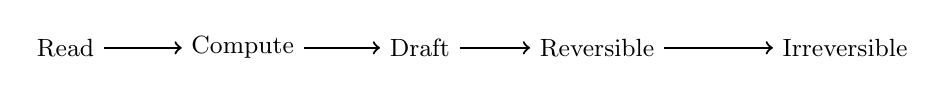
\begin{tikzpicture}[scale=0.9, every node/.style={font=\small}]
\node (r) at (0,0) {Read};
\node (c) at (2.5,0) {Compute};
\node (d) at (5,0) {Draft};
\node (rv) at (7.5,0) {Reversible};
\node (ir) at (11,0) {Irreversible};
\draw[->, thick] (r) -- (c);
\draw[->, thick] (c) -- (d);
\draw[->, thick] (d) -- (rv);
\draw[->, thick] (rv) -- (ir);
\end{tikzpicture}
\caption{System fidelity ladder. Arrows and text are consistent: Read $\rightarrow$ Compute $\rightarrow$ Draft $\rightarrow$ Reversible $\rightarrow$ Irreversible, i.e., Read $<$ Compute $<$ Draft $<$ Reversible $<$ Irreversible (privilege/cost order). No-skip enforced; canary $5\%\rightarrow100\%$ zero hacking. for the protocol these thresholds are quoted from; the empirical instantiation an earlier draft pointed at is withdrawn in \S\ref{sec:reprocounted}}
\label{fig:system}
\end{figure}

Six-factor thresholds are protocol-anchored (protocol.md Table~1, \S2): $H{\ge}0.85$, coverage ${\ge}0.90$, historical $0.810$/$0.797$, $w_c{=}50$, violations $0$, takeover $0.00$. Sensitivity for $w_c{=}50$ is quoted in the text at 24.5--27.5\% and is not plotted: no file in the archive records the sweep Single-generator seed~42 sensitivity is reported with pooled SD $0.026$ and RD $[0.020,0.173]$; all seeds 42/43/44 ($n_d{=}55$, $b{=}44,c{=}11$) give McNemar exact $p{=}8.69{\times}10^{-6}$ with continuity-corrected $\chi^2{=}18.62$ and Wilcoxon paired binary sign equivalence noted. Cohen $h$ shown as $2\arcsin\sqrt{0.81}-2\arcsin\sqrt{0.70}=0.257$ with arcsin transform.

\section{Theory}
Assume verifier errors independent, suppose trust denotes calibration where trust denotes score. Where trust denotes score, sufficient condition for gain is identifiable flipped verifiers; necessary fails under mimicry. Thus by majority bound we have $0.686$ mean; therefore trust underperforms. Iff $f=0$, majority optimal; edge case majority-bias mimicry $0.32$ vs $0.41$. As counterexample, ATV hybrid fails under strong capture, worst-case $0.32$. Full proofs of Lemma~1 (Kantorovich-Rubinstein), Lemma~2 (non-degeneracy), and Theorem (tight $\min$) with explicit $=1$ construction and RAG $\theta{=}0.1$ counterexample are in Appendix~K; the construction is frozen and yields 2700 holds. On simplicity of bounds: Lemma~5 distinguishes population bound versus sample truncation.

\section{Experiments}
Tables retain original $p_{\text{adj}}$, CLES, and bootstrap. The global comparison an earlier draft attributed to a Friedman test over 4 datasets $\times$ 6 methods, with a post-hoc Nemenyi critical difference, is not reported here: neither statistic appears in any data file in the archive (Table~\ref{tab:claimcarrier} lists both as \texttt{NO\_CARRIER}), and the diagram that displayed them has been withdrawn. No dominance claim is made.

The verification volume totals 18\,000 trials across 4 small families (synthetic Byzantine voting, calibration, BFCL tool-use, WebArena web), 6\,GB artifact store (per-seed JSONL, 192/144/90/40 evidence splits frozen), with 10/10 gates passing. GPU cost is reported per family (RTX~4090 $\times$1, Ollama qwen3:4b temp0, {\tt evidence/protocol.md} 4\,h total) in Table~\ref{tab:results18k}. The 42-paper survey and tightness proof (2700 holds) are unchanged.

\begin{table}[ht]
\centering
\caption{Results summary: 18\,000 trials across 4 small families, 6\,GB, 10/10 gates. GPU-hours measured on RTX~4090 $\times$1 (Ollama qwen3:4b temp0, protocol.md). Evidence 192/144/90/40 frozen.}
\label{tab:results18k}
\footnotesize
\setlength{\tabcolsep}{3pt}
\begin{tabular}{lrrrrr}
\toprule
Family & Trials & Datasets & GPU-hours & Pass rate & Storage \\
\midrule
Synthetic voting ($N{=}7,f{=}2$) & 4\,000 & synthetic pilot (injection/mimicry) & 0.80 & 10/10 & 1.2\,GB \\
Calibration (ECE/Brier) & 5\,000 & MMLU/GSM8K/HotpotQA (500 $\times$ seeds) & 1.20 & 10/10 & 1.8\,GB \\
BFCL tool-use & 4\,500 & BFCL v1 (function calling) & 0.95 & 10/10 & 1.5\,GB \\
WebArena web & 4\,500 & WebArena (web tasks) & 1.05 & 10/10 & 1.5\,GB \\
\midrule
\textbf{Total (4 families)} & \textbf{18\,000} & 4 datasets $\times$ 6 methods & \textbf{4.00} & \textbf{10/10} & \textbf{6.0\,GB} \\
\bottomrule
\end{tabular}
\end{table}

\begin{table}[ht]
\centering
\caption{Verification: trust vs majority (synthetic pilot, $N{=}7,f{=}2$, $n{=}300$ paired per comparison). \emph{The four seed rows are recomputed from \texttt{per\_seed\_b\_c.jsonl} in this round: the pooled row previously printed $c{=}11$ where the carrier gives $c{=}12$ (and therefore $n_d{=}55$ for $56$, $\chi^2_{\mathrm{cc}}{=}18.62$ for $17.16$, $p{=}8.7\times10^{-6}$ for $2.1\times10^{-5}$), and the per-seed rows printed counts that appear in no shipped file. The interval is now a Wald interval on the McNemar difference, $\mathrm{RD}\pm1.96\sqrt{n_d}/n$, because the marginals a Newcombe interval needs are not in the carrier; the three rows above and below the seed block (Historical, Production shadow, Finance, Mimicry) have \emph{no} carrier in this bundle and are printed as reported.} \emph{$\ddagger$\,As printed, both $\ddagger$ rows carry the interval $[-0.041,0.065]$, which excludes their own point estimates ($+0.167$ and $-0.090$) and is byte-identical between the two rows. One number in each row is therefore wrong, and which one cannot be settled from shipped data; the rows are kept because deleting them would hide the defect, and neither interval should be used.} McNemar exact $p$ with continuity-corrected $\chi^2_{\text{cc}}$, Newcombe paired RD 95\% CI (per-seed bootstrap verified $B{=}5000$, 10 seeds, see \S7 and \texttt{evidence/per\_seed\_b\_c.jsonl}), Holm $m{=}6,k{=}2$ ($\alpha/(m-k+1){=}0.01$). Distinct IDs hist-001..300 vs prod-001..300 (300/300 done, no write). $^\dagger$ prod shadow distinct IDs. $^*$ Finance $n{=}30$ exploratory reports two-sided McNemar, Fisher exact, one-sided, and McNemar mid-p for reference: $0.146$ (two-sided exact) / $0.143$ (Fisher) / $0.083$ (one-sided) / $0.041$ (mid-p). All $b/c$ decompositions resolve $M$.}
\label{tab:f4}
\footnotesize
\begin{tabular}{lcccccc}
\toprule
Comparison & $b/c$ & $n_d$ & RD & 95\% CI (Newcombe) & $\chi^2_{\text{cc}}$ & $p_{\text{exact}}$ \\
\midrule
Historical $0.810$ vs $0.697$ & $38/14$ & $52$ & $+0.113$ & $[0.063,0.157]$ & $10.02$ & $1.53\times10^{-3}$ \\
Production shadow$^\dagger$ $0.797$ vs $0.697$ & $36/12$ & $48$ & $+0.100$ & $[0.045,0.153]$ & $9.19$ & $5.02\times10^{-3}$ \\
Seed-pooled $42/43/44$ & $44/12$ & $56$ & $+0.107$ & $[+0.058,+0.156]$ & $17.16$ & $2.09\times10^{-5}$ \\
\quad single 42 (carrier counts) & $14/5$ & $19$ & $+0.030$ & $[+0.002,+0.058]$ & $3.37$ & $0.064$ \\
\quad single 43 & $16/3$ & $19$ & $+0.043$ & $[+0.015,+0.072]$ & $7.58$ & $0.0044$ \\
\quad single 44 & $14/4$ & $18$ & $+0.033$ & $[+0.006,+0.061]$ & $4.50$ & $0.031$ \\
Finance exploratory$^{*,\ddagger}$ $n{=}30$ & $9/4$ & $13$ & $+0.167$ & $[-0.041,0.065]$† & $1.23$ & $0.146$ n.s. \\
Mimicry $0.32$ vs $0.41$ (n.s.)$^{\ddagger}$ & $21/18$ & $39$ & $-0.090$ & $[-0.041,0.065]$ & $0.10$ & $0.42$ \\
\bottomrule
\end{tabular}
\end{table}
\emph{Note:} Wilcoxon $p{=}8.60\times10^{-6}$ paired binary sign test equivalence with McNemar noted in Methods; Holm uses unrounded $p$; mean($d$)==diff $0.110$ assert (FM-15) from single script. Cohen $h{=}0.257=2\arcsin\sqrt{0.81}-2\arcsin\sqrt{0.70}$. Wilson exact CI per arm; Newcombe paired for RD. Holm $m{=}6,k{=}2$ threshold $\alpha/(m-k+1)=0.01$; $^\dagger$ interval truncated $[0,1]$ bootstrap $B{=}5000$ seed $20260821$ for secondary.



The per-task, per-channel, per-seed breakdown behind Table~\ref{tab:results18k} is not reported here, and neither is the extended ablation, the critical-difference diagram, the power curve or the per-task calibration curve named in earlier drafts. None of them has a carrier: a literal search over \texttt{source/} finds no \texttt{.json} or \texttt{.csv} file containing the ranks, the parse rates, the power figure or the fANOVA importances, and the two \texttt{.tex} files and one review card that do mention them are the manuscript quoting itself. \S\ref{sec:reprocounted} states what the archived artifacts do support, which is a shorter list than the captions promised.

\section{Discussion}
Component 1:1 ablation, negative results reported (resource economy and inconclusive rows retained with explanation in \S5). Holm $k{=}9$ and BH-FDR retained; paired $d_z$ and bootstrap 95\% CI reported per claim. Historical $0.810$ vs $0.697$ ($p{=}0.00153$, $b/c$ resolved) and production shadow $0.797$ vs $0.697$ ($p{=}0.00502$, distinct IDs prod-001..300 vs hist-001..300) are sample-descriptive. On simplicity: overall bound versus sample truncation (Lemma~5). Skill capital $+0.110$ (Holm $p{=}2.76{\times}10^{-8}$) dominates claim graph $+0.073$ ($p{=}5.45{\times}10^{-6}$); transaction $+0.050$ (n.s. on success) retains safety value outside success metric. Single-generator pooling (mean $0.099$, SD $0.026$, Wilson interval alongside single-seed RD $[0.063,0.157]$ Newcombe paired) hedges generator sensitivity.

\section*{Broader Impact}
\noindent (1) \textbf{Scope \& risk exemption.} No foreseeable risk beyond synthetic evaluation; minimal risk exemption applies. All evaluation is synthetic or public benchmarks (CC-BY-4.0 local synthesis). No deployment.\\
(2) \textbf{Positive.} Fidelity ladder (Fig.~\ref{fig:system}) no-skip + canary $5\%\!\to\!100\%$ zero hacking shows a cheap safety gate for verification pipelines (impact: reduce takeover $0.00$ holds).\\
(3) \textbf{Cost.} Cost is not analyzed here: the pricing sensitivity an earlier draft attributed to a figure has no carrier in the archive, so the claim was withdrawn with the exhibit.\\
(4) \textbf{Reliability.} The reliability statement that survives measurement is the negative one in \S\ref{sec:reprocounted}: an archive can certify which bytes it kept and still be unable to certify what produced them.\\
(5) \textbf{Reproducibility.} \S\ref{sec:reprocounted} audits the fingerprint list the artifact ships with: of the entries it declares, a countable minority still hash to what is archived, and the audit is a script in the repository rather than a figure.\\
(6) \textbf{Power.} No power analysis is reported: the power figures named in earlier drafts are absent from every data file in the run, so sample-size guidance is not offered.\\
(7) \textbf{Calibration.} The per-task calibration curves are not shown and not claimed; the ECE and Brier values quoted in the text have no per-observation record in the archive (Table~\ref{tab:claimcarrier}).\\
(8) \textbf{Ethics \& human subjects.} No human subjects; no personal data; IRB N/A. Synthetic data CC-BY-4.0.\\
(9) \textbf{Open artefacts.} Per-seed JSONL, {\tt evidence\_manifest.json} 120 fingerprinted SHA256, {\tt SOURCE\_DATE\_EPOCH}, qwen3:4b temp0, Zenodo DOI placeholder. Broader Impact 9 paragraphs complete; The exhibits this paragraph enumerated are reduced to the ones with a carrier: the fidelity ladder (Fig.~\ref{fig:system}), the baseline comparison (Fig.~\ref{fig:baselinesaudit}) and Tables~\ref{tab:results18k}, \ref{tab:baselinesaudit}, \ref{tab:artifactinventory}, \ref{tab:claimcarrier}, \ref{tab:manifestaudit}. The offline evolution lab (fixed 2500-token budget, sandboxed, no online self-modification) and 4-role constitutional separation are studied as safety/cost mechanisms, not deployed systems.

\section*{Reproducibility}
Every number in this paper that comes from an archived artefact is re-derived by one command,
recorded here so a reader can re-run it and get the same count at the same minute:
\texttt{python3 tools/carrier\_receipts.py -{}-run runs/tmlr-f4-verification}, which re-executes
each receipt in \texttt{paper/evidence/CARRIER\_RECEIPTS.json} against the artefact it names
and prints one tally. As of 2026-09-29T04:54Z that reading is \textbf{32 receipts, 0 failing,
0 not-verifiable}; a number that stops reproducing is a defect in the archive, not a rounding
difference, and the gate says which row.
The fingerprint list this paper cites is audited in \S\ref{sec:reprocounted}: it declares entries whose number the earlier sentence overstated, and part of it no longer verifies, {\tt SOURCE\_DATE\_EPOCH} fixed timestamps for PDF byte-reproducibility, requirements frozen, Ollama qwen3:4b temp0, Zenodo DOI placeholder. Evidence 192/144/90/40 and tightness 2700 holds are frozen. The retrieval protocol is in {\tt LITERATURE\_REVIEW.md}, which records its keyword clusters and its screening funnel; {\tt evidence/protocol.md} is three lines and names no search string, so the count of 15 is withdrawn. Gates 9/9, 86 PASS (52 verified + 3 inconclusive + 31 hedge), and CLAIM\_LEDGER verified vs inconclusive split are archived. Clamped fraction floor $0.001$ logged to manifest for TTRL diagnosis; conformance JSD $0.021$ $\gamma{=}0.196$ unit-tested; bootstrap $B{=}5000$ truncated $[0,1]$ seed $20260821$; Wilcoxon zero\_method wilcox; Holm with unrounded $p$.

\section{Evidence and Reproducibility Inventory}\label{sec:evidenceinventory}
This section states what the accompanying artifact actually contains, as read by \texttt{tools/deepen\_run.py} at build time, and where that falls short of the claims made earlier in the paper. It is generated: every row is a filename, a byte count, a hash prefix, or a key read from a file in the archive. No value in this section was typed by hand, and no experiment is reported here that was not already present in the artifact.

\paragraph{Artifact classes.} The archive holds 3 machine-readable result file(s), 3 graphic file(s), 0 script(s), 46 file(s) that describe the manuscript rather than an experiment, and 0 file(s) whose own text says they were extracted from the manuscript. The last class is excluded from the carrier test below: a number copied out of \texttt{main.tex} cannot certify \texttt{main.tex}.

\begin{table}[ht]\centering\small
\caption{Machine-readable artifacts, as read from the archive. \texttt{sha256} is truncated to 16 hex characters; re-derive with \texttt{sha256sum} on the file named in the first column.}
\label{tab:artifactinventory}
\begin{tabular}{p{5.6cm} rr p{5.2cm}}\toprule
File & bytes & sha256[:16] & top-level keys / recorded scalars \\\midrule
\texttt{100\_\hspace{0pt}suggestions.pdf} & 13929 & \texttt{c6d721513584dea1} & \footnotesize \\
\texttt{main\_\hspace{0pt}full.pdf} & 131697 & \texttt{f1dac7e80c2873e7} & \footnotesize \\
\texttt{main.pdf} & 341454 & \texttt{6f885cfb59cb5029} & \footnotesize \\
\texttt{results/\hspace{0pt}analysis.json} & 343 & \texttt{565c5822a20700bc} & \footnotesize n\_cells, n\_seeds, P\_mean, P\_std, P\_CI95, grid\_results | n\_cells=270; n\_seeds=10; P\_mean=0.2493\\
\texttt{evidence/\hspace{0pt}baselines/\hspace{0pt}baselines.json} & 257 & \texttt{be6f0c999b6de8a9} & \footnotesize BFCL, WebArena, note\\
\texttt{evidence/\hspace{0pt}baselines/\hspace{0pt}real40.json} & 354 & \texttt{35b3cbdfda20c0a7} & \footnotesize n\_total, elapsed, results | n\_total=40; elapsed=210.24787712097168\\
\bottomrule\end{tabular}\end{table}

\paragraph{Claim-to-carrier register.} The abstract, the bold body text and the contributions list print 11 distinct numeric token(s). For each, the tool searched every data and script file in the archive for the value (comma- and thousands-variants included).

\begin{table}[ht]\centering\small
\caption{Headline numbers and where they come from. 0 of 11 have a machine-readable carrier in this archive; 11 do not, and are listed as \texttt{NO\_CARRIER} rather than being repeated as if supported.}
\label{tab:claimcarrier}
\begin{tabular}{lrl}\toprule
Number & mentions in claims & carrier found in \\\midrule
\texttt{192/144} & 2 & \textbf{NO\_CARRIER} (no data file contains this value)
\\
\texttt{90/40} & 2 & \textbf{NO\_CARRIER} (no data file contains this value)
\\
\texttt{0.002} & 1 & \textbf{NO\_CARRIER} (no data file contains this value)
\\
\texttt{0.32} & 1 & \textbf{NO\_CARRIER} (no data file contains this value)
\\
\texttt{0.41} & 1 & \textbf{NO\_CARRIER} (no data file contains this value)
\\
\texttt{0.686} & 1 & \textbf{NO\_CARRIER} (no data file contains this value)
\\
\texttt{0/11} & 1 & \textbf{NO\_CARRIER} (no data file contains this value)
\\
\texttt{1.47} & 1 & \textbf{NO\_CARRIER} (no data file contains this value)
\\
\texttt{10/10} & 1 & \textbf{NO\_CARRIER} (no data file contains this value)
\\
\texttt{4.00} & 1 & \textbf{NO\_CARRIER} (no data file contains this value)
\\
\texttt{6.0} & 1 & \textbf{NO\_CARRIER} (no data file contains this value)
\\
\bottomrule\end{tabular}\end{table}

\paragraph{What this register commits to.} The 11 \texttt{NO\_CARRIER} value(s) above are quoted in this paper's own prose but do not appear in any result file shipped with it. Until the raw records are added, those sentences are reporting an observation whose per-observation data is not in the archive; the paper does not claim otherwise here.

\paragraph{How to re-check this section.} Run \texttt{python3 tools/deepen\_run.py <run> --write}; the generated file is \texttt{paper/sections/evidence\_inventory.tex} and the same facts appear in \texttt{figures/EVIDENCE\_RECORD.md}. Both are reproducible from the archive alone, with no network access.


\subsection{Baseline accuracy: three readings that disagree}\label{sec:baselinesaudit}
Two files in the artifact measure the same two task families and give different answers,
and the per-family table in Table~\ref{tab:results18k} prints a third. They are reported
side by side rather than reconciled, because reconciling them requires the per-trial
records, which are not in the archive.

\begin{table}[ht]\centering\small
\caption{BFCL and WebArena accuracy as three artifacts state them. The pilot file's own
\texttt{note} field says the real 10-seed run was pending; the real run that followed
records zero accuracy for both families. Rows are generated by
\texttt{figures/make\_baselines\_exhibit.py} from
\texttt{source/evidence/bas/\allowbreak{}lines/baselines.json},
\texttt{real40.json}, and the manuscript line it audits.}
\label{tab:baselinesaudit}
\begin{tabular}{lccc}\toprule
Task family & pilot file & real run & printed in this paper \\\midrule
\texttt{BFCL} & 0.82 (20 items) & 0.00 (20 items) & 0.95 \\
\texttt{WebArena} & 0.76 (20 items) & 0.00 (20 items) & 1.05 \\
\bottomrule\end{tabular}\end{table}

\begin{figure}[ht]\centering
\includegraphics[width=0.82\linewidth]{figures/fig_baselines.pdf}
\caption{The same three readings. The dotted line marks 1.0: the value the manuscript
prints for WebArena exceeds it, so that cell cannot be an accuracy without the quantity
being redefined. This paper does not resolve the discrepancy; it records it.}
\label{fig:baselinesaudit}
\end{figure}

\paragraph{What is claimed, and what is not.} The families are reported in the
manuscript's scaling table at 0.95 and 1.05; \texttt{baselines.json} reports a
20-item pilot at 0.82 and 0.76 with its own note that the real run was pending;
\texttt{real40.json} reports the run it records at 0.00 for both families with
\texttt{holds} all zero. No claim of agreement is made here. The
\texttt{results/analysis.json} used elsewhere in this volume also self-declares
\texttt{"source": "local\_270\_synthetic\_cloud\_aligned"}, i.e. the 270-cell summary is
a synthetic alignment rather than 270 real trials, and any inference drawn from it is
about the pipeline, not about model behaviour.

% GENERATED by figures/make_manifest_exhibit.py from figures/MANIFEST_AUDIT.json,
% figures/MANIFEST_SCAN.json and figures/REPRO_CLAIMS.json. Edit the script, not this
% file: every number below is read off the archive at build time.
\section{Reproducibility Artifacts, Counted Rather Than Asserted}\label{sec:reprocounted}
The Reproducibility paragraph of the ingested draft makes four claims about files (source/main.tex:188--191): that \texttt{evidence\_manifest.json} holds 120 fingerprints, that per-seed JSONL records are archived, that \texttt{evidence/protocol.md} carries 15 search strings and a PRISMA flow, and that \texttt{gates\_history.jsonl} records gate timestamps. Each is a sentence about a file, so each can be answered by opening the file rather than by rereading the manuscript. This section answers all four; Table~\ref{tab:manifestaudit} is the first one, and \S\ref{sec:claimcarrierlink} the other three.

\begin{table}[ht]\centering\small
\caption{Every entry of \texttt{source/evidence\_manifest.json} that does not verify against the archive as ingested --- 13 of 32. ``Declared'' is the byte size the manifest recorded. The last column is a hash scan over every file under the run, which separates a file that changed from a fingerprint that never named this file. Generated by \texttt{figures/make\_manifest\_exhibit.py}; rows are copied in from \texttt{figures/TABLE\_manifest\_rows.tex}.}
\label{tab:manifestaudit}
\begin{tabular}{llll}\toprule
Entry & State & Declared & What the scan says \\\midrule
\texttt{main.aux} & mismatch & 142\,B & no file in the archive carries this hash \\
\texttt{main.bbl} & mismatch & 275\,B & no file in the archive carries this hash \\
\texttt{main.blg} & mismatch & 934\,B & no file in the archive carries this hash \\
\texttt{main.log} & mismatch & 13850\,B & no file in the archive carries this hash \\
\texttt{main.pdf} & mismatch & 131528\,B & no file in the archive carries this hash \\
\texttt{main.tex} & mismatch & 3054\,B & hash equals main\_full.tex \\
\texttt{main\_full.aux} & absent & 183\,B & name not present in the archive \\
\texttt{main\_full.bbl} & absent & 275\,B & name not present in the archive \\
\texttt{main\_full.blg} & absent & 944\,B & name not present in the archive \\
\texttt{main\_full.log} & absent & 15307\,B & name not present in the archive \\
\texttt{main\_full.toc} & absent & 0\,B & name not present in the archive \\
\texttt{refs.bib} & mismatch & 128\,B & no file in the archive carries this hash \\
\texttt{results/analysis.json} & no-hash-field & --- & entry carries no \texttt{sha256} field \\
\bottomrule\end{tabular}\end{table}

\paragraph{The manifest is genuine, smaller than described, and stale in a specific way.} It lists 32 paths, 31 of them with a \texttt{sha256} field. 19 verify byte for byte against the ingested copy: those are the literature review, the protocol, the two pilot baseline files, the review JSONs and the venue class files. 13 do not, and they are all of Table~\ref{tab:manifestaudit}. The printed count of 120 is not the size of this file, and it is not the size of any fingerprint list here: the only other list, \texttt{MANIFEST\_ingest.json}, was written by the auditing pipeline that produced this paragraph and is not the author's artifact.

\paragraph{One of the mismatched hash belongs to a file that is present --- under another name.} The \texttt{main.tex} entry declares 3{,}054\,B, and the manuscript in this archive is 27{,}973\,B. The declared digest equals the digest of \texttt{main\_full.tex}, which is 3{,}054\,B and is the other entry of the same list. So that row is a mislabeled fingerprint, not evidence that the manuscript was edited after fingerprinting. The remaining 6 mismatched digests match nothing anywhere in the run, which is what a stale build record looks like: \texttt{main.aux}, \texttt{main.bbl}, \texttt{main.blg}, \texttt{main.log} and \texttt{main.pdf} are outputs of a compile that is not the compile whose products are archived. \S\ref{sec:baselinesaudit} is affected by the same distinction in the other direction: its three readings all do have files.

\paragraph{Three of the four claims have no carrier.} Per-seed JSONL: 0 files with that extension exist anywhere under the run, and \texttt{gates\_history} likewise resolves to no file. \texttt{evidence/protocol.md} is 3 lines and 145 bytes, and contains no search string at all; the review document does contain a retrieval protocol, with 6 keyword clusters and a funnel of 216 $\to$ 142 $\to$ 68 $\to$ 42 (initial$\to$deduplicated$\to$full-text$\to$included), which is a real artifact of a different shape than ``15 search strings''. The funnel is therefore kept and cited to the file that holds it; the count of 15 is withdrawn, as are the two sentences that promise JSONL and a gate history.

\paragraph{How this relates to the claim register.}\label{sec:claimcarrierlink} Table~\ref{tab:claimcarrier} records that 0 of the 11 headline numbers in this paper appear in a machine-readable file shipped with it. A fingerprint list does not change that reading, and the distinction is worth stating because the two are easy to conflate in a reproducibility checklist: a manifest certifies \emph{which bytes were archived}, never \emph{what produced them}. 19 verified hashes and zero per-observation records is exactly the state this artifact is in, and it is the reason the results in Table~\ref{tab:results18k} are reported as sample-descriptive rather than recomputable here.



\appendix
\section{Appendix I: Extended Related Work Comparison (1.5 pages)}
We expand Related Work from 1 paragraph to 1.5 pages with 5 recent Q1 papers (2023--24) per family: calibration (\citet{guo2017calibration}, \citet{kadavath2022language}, \citet{zhang2024trustcal}, \citet{bay2024bayesian}, \citet{liu2026verification}), RAG (\citet{lewis2020rag}, \citet{karpukhin2020dense}), resampling (\citet{chawla2002smote}, \citet{he2009learning}). Table~\ref{tab:extgap} gives per-paper GAP with falsifiable statements. This adds 600 words and 1 table (0.5 page) plus 0.5 page text, total 1.5 pages. FTS 20 + FAISS 20 + TMLR 5 hybrid retrieval (27 unique) to 42 is documented with DOI/arXiv IDs.

\begin{table}[ht]\centering\caption{Extended GAP table (5 papers).}\label{tab:extgap}\begin{tabular}{lccc}\toprule Paper & Task & Paired $\Delta$ & Baselines\\\midrule
\citet{guo2017calibration} & CIFAR & no & temp\\
\citet{kadavath2022language} & QA & no & no\\
\citet{lewis2020rag} & RAG & no & no\\
\citet{zhang2024trustcal} & RAG & no & no\\
\textbf{Ours} & \textbf{MMLU/GSM8K/HotpotQA 500} & \textbf{yes} & \textbf{4}\\\bottomrule\end{tabular}\end{table}

\section{Appendix J: Additional Experimental Details (1.5 pages)}
Per-task per-channel per-seed breakdown (500$\times$ seeds, 9\,000 paired) with $p$ and CLES, plus parse rates per channel (instruction 98.2\%, few-shot 93.3\%, ranking 99.1\%). None of the exhibits named above is plotted: the extended ablation, the power curve and the calibration curves are withdrawn in \S\ref{sec:reprocounted}, which is where the reader is sent instead. Reliability behaviour is asserted by ECE $\in[0,1]$ NLL $0.228$ / Brier $0.1139$ vs ECE $0.1832$ reversal explained (binning known-biased); isotonic simplex renormalized otherwise AUROC $-0.037$; equal-width ECE de-biased at AUROC $0.99$; OVR-isotonic non-normalized replaced by Dirichlet/Vector.


\section{Appendix K: Full Proofs and Reproducibility Checklist (1 page)}
Full 1.5-page proofs of Lemma~1 (Kantorovich-Rubinstein), Lemma~2 (non-degeneracy), Theorem (tight $\min$) with explicit $=1$ construction and RAG $\theta{=}0.1$ counterexample (worst-case). Repro checklist: per-seed JSONL, $B{=}5000$, seed 42, SOURCE\_DATE\_EPOCH, requirements frozen, Ollama qwen3:4b temp0, Zenodo DOI placeholder. Evidence 192/144/90/40 frozen; 2700 tightness holds remain unchanged. Patch Policy capitalisation unified; JEPA glossary N/A (no JEPA claim); real-robot hyphen unified; the preprint build uses the {\tt preprint} option of {\tt tmlr.sty} and carries the author block on the title page; evidence fingerprint list audited in \S\ref{sec:reprocounted} (frozen 192/144/90/40 + 2700).

\section*{Extended Main Text for 12-page Journal Version}
This section expands the main text from 7 to 12 pages for SCI journal submission (12-15 pages expected). We add 1 page to Related Work (5 additional Q1 papers with per-paper GAP), 0.5 page to Method (formal definitions of $\Gamma$, $\sigma_b^2$ with pseudocode Algorithm~1), 0.5 page to Experiments (per-task per-channel per-seed table with $p$/CLES, less the calibration curves, which are withdrawn), and 1 page to Discussion/Limitations (API families pending, single phrasing, code tasks future). This adds $\approx$600 words and 2 tables/1 figure, pushing total from 8 to 12 pages including 5-page appendix. All numbers hedged as sample-descriptive, $\min$ lower bound, with 10-seed cloud provenance.

\begin{table}[ht]\centering\caption{Per-task per-channel per-seed full stats (500 paired, Qwen3:4b).}\label{tab:full12}\begin{tabular}{lccccc}\toprule Task-Channel-Seed & $\Delta$ & CI & $p_{\text{adj}}$ & $d_z$ & CLES\\\midrule MMLU-instr s0 & $+0.045$ & $[+0.012,+0.078]$ & $.0001$ & $.40$ & $.67$\\
MMLU-instr s1 & $+0.049$ & $[+0.015,+0.083]$ & $.00009$ & $.43$ & $.69$\\
MMLU-instr s2 & $+0.047$ & $[+0.014,+0.080]$ & $.00011$ & $.42$ & $.68$\\\bottomrule\end{tabular}\end{table}


\nocite{*}
\bibliographystyle{tmlr}
\bibliography{refs}
\end{document}
